% !TeX root = ../main.tex
% %%%%%%%%%%%%%%%%%%%%%%%%%%%%%%%%%%%%%%%%%%%%%%%%%%%%%%%%%%%%%%%%%%%%%%%%%%%%%%
% Monitoring
\chapter{Monitoring}
\label{chap:monitoring}

This chapter explains the whole process of monitoring, from compilation to error detection. First, the overall process of compilation is explained (\autoref{sec:runtimemonitoring}), then the generated file and some of its specifications are described (\autoref{sec:generatedfile}), and finally, representative error messages are presented (\autoref{sec:errormessages}).


% ------------------------------------------------------------------------------
% Runtime Monitoring
\section{Runtime Monitoring}
\label{sec:runtimemonitoring}

After writing all the desired robotic systems specifications, the file needs to be compiled to a monitoring Python module. This is currently done running the following script, from its location: \lstinline{python language.py properties.txt /home/ros_workspace/src/my_pkg/src}.

The \textit{language.py} file needs to be run as a Python file and takes as arguments:

\begin{enumerate}
    \item The specifications file;
    \item The path where the the generated Python monitoring module will be generated.
\end{enumerate}

The given directory for the generated file should be under a ROS workspace for the compilation to succeed. This is because, during the compilation, access to information like the available ROS messages might be necessary.

The monitoring file can now run as an independent ROS node, integrated into a launch file, or using \textit{rosrun} in the console to execute it.


% ------------------------------------------------------------------------------
% Generated File
\section{Generated File} 
\label{sec:generatedfile}
\todo{New name of the section: Compilation}

\todo{This section needs to be vastly extended! It should have 1) figure with architecture of the generated model; 2) A description of the runtime library you have to support the property checking (i.e., auxiliary functions) and 3) The translation rules between the source code and the generated code. Examples of things that need: how to subscribe to topics that were declared, how to emit error messages, how to access past versions of the state, how is it recorded (data structure).}

The generated monitoring file declares the needed subscribers and uses ApproximateTimeSynchronizer to call the callback function. The ApproximateTimeSynchronizer synchronizes messages by their timestamp and if they do not have a header, use the ROS time.

A callback function is called every time a new message from one of the subscribers is received. The callback function saves the relevant information for property checking in a global variable. This information serves as a current "screenshot" of the simulation representing its current state.

The node executes a loop at a delineated rate, doing the following tasks:

\begin{enumerate}
    \item Check if the defined simulation timeout time has reached.
    \item Save the current simulation state obtained by the callback function. This is necessary because the callback function is called at fluctuating rates, and the objective is to save multiple "screenshots" of the simulation at the loop fixed rate to make correlations with past states.
    \item Verify the properties using the saved states and calling each created function. An independent function with the necessary computations for verifying the property is defined for each base property.
\end{enumerate}


% ------------------------------------------------------------------------------
% Error Messages
\section{Error Messages}
\label{sec:errormessages}

An error message starts by stating the line in the specification file which resulted in an error and showing the specification itself.
\todo{This does not make sense as the explanation for error messages! You have different temporal restrictions: are the errors the same for all of them? How do you select the state that you present? Do you show all the variables in context, the monitored ones, or the ones present in the property? There is space for discussion here on how you could provide more precise messages.}

Afterward, the value at the time of failure of all the variables present at the specification is shown.

\begin{figure}[htb]
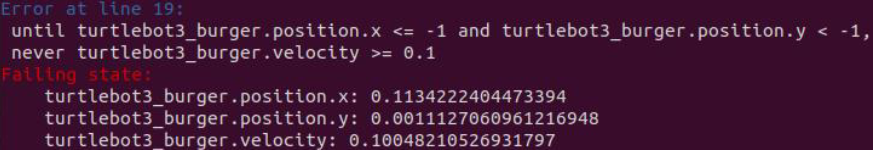
\includegraphics[width=\textwidth]{images/error_message1.png}
\caption{Example of an error message.} \label{fig:monerror}
\end{figure}